\documentclass[10pt, a4paper, oneside]{article}

\usepackage[english]{babel}
\usepackage{amsfonts}
\usepackage{amsmath}
\usepackage{amssymb}
\usepackage{hyperref}
\usepackage[latin1]{inputenc}
\usepackage{graphicx}

\begin{document}
\title{Topic Grouper - An Alternative Computational Approach in the Field of Probabilistic Topic Modeling}
\author{Daniel Pfeifer, Hochschule Heilbronn (Germany)}
%\date{} %%Wenn kommentiert, wird das aktuelle Datum verwendet.
\maketitle

\section{Introduction}

This document is work in progress. It presents the basic concepts of a new approach for topic modeling. This new approach, called "Topic Grouper", essentially combines a generative stochastic perspective on topic computation with agglomerative clustering.
As opposed to conventional clustering approaches for document collections, Topic Grouper essentially establishes a cluster distance on topics instead of documents. 

Topic Grouper starts with one-word-topics, of which there are as many as words in the vocabulary. At every step, it selects the topics "closest" to each other and joins them. This way topics, i.e. sets of words, remain disjunct at every step. The algorithm ends at the point where there is just one topic left -- the union of all words in the vocabulary.
On the way there, it provides a solution for every possible number of disjunct topics (ranging between the vocabulary size $|V|$ and $1$).

The corresponding cluster distance measure is derived by considering documents to be generated via a stochastic process over disjunct topic sets. This is a principal quality that Topic Grouper shares with "purer" statistical approaches such as LDA \cite{Blei:2003:LDA:944919.944937} and its variants.
The generative model of Topic Grouper lends itself well to apply clustering in reasonably efficient way (see Section \ref{basics}). It is simple and intuitive but differs from the generative model behind LDA and its variants: Since with Topic Grouper, words get hard-assigned to topics, there is no need to statistically infer "word per topic distributions" or "topic per document distributions". Nevertheless, the importance of words in a topic can be determined directly by corresponding word frequencies as given via the corpus. Analogously, the influence of topics per document can determined as well.

\subsection{Clustering and Topic Modeling}

Document clustering is obviously very popular and has been under consideration since the early days of information retrieval \cite{Salton:1975:VSM:361219.361220}. However applying clustering to topics directly, i.e. the latent topics in documents and document collections, seems to be a new approach.
\cite{wallach08} discusses clustering and topic modeling in Chapter 5 but only with regard to clustering documents -- not topics.

\subsection{Hyperparameters and LDA}

In comparison to LDA (which is the predominant approach in probabilistic topic modeling), Topic Grouper is much less susceptible to the choice of hyperparameters. In fact, in its basic variant, Topic Grouper works without any hyperparameters at all. In contrast, classical LDA mandates the setting of the number of topics $n$ and two vectors $\alpha \in \Re^n$ and $\beta \in \Re^{|V|}$ with $|V|$ being the vocabulary size. Finding "good" values for those LDA-related hyperparameters is anything but trivial. A body of scientific work has been created around this issue including:
\begin{itemize}
\item a generalization of LDA to compute $n$ as part of an enhanced generative model (\cite{Teh04hierarchicaldirichlet}),
\item a generalization of LDA to compute $\alpha$ as part of a generative model (\cite{conf/nips/WallachMM09}), also showing that the choice of a symmetric $\beta$ using a default value is usually sufficient,
\item adapting LDA such that it is less susceptible to the choice of $\alpha$ (\cite{Tan_topic-weak-correlatedlatent}),
\item defining measures for hyperparameter search and selection with regard to $n$ (\cite{Arun2010}),
\item avoiding heavily differing topic probabilities (affecting the choice of $\alpha$) by filtering stop words or including a background model (\cite{conf/nips/ChemuduguntaSS06}).
\end{itemize}

\subsection{State of Knowledge on Topic Grouper}

Using synthetic data sets according to \cite{Tan_topic-weak-correlatedlatent} Topic Grouper has already shown
\begin{itemize}
\item to work reasonably efficient on these date sets,
\item to offer good solutions for these data sets (returning close to "perfect" solutions),
\item to offer good solutions in the case of differing topic probabilities (in which case classical LDA fails when using a symmetric prior $\alpha$, as often done in practice),
\item to allow for picking the correct (or a reasonable) number of topics via a simple inspection of a so-called "likelihood improvement graph". (The latter can easily be generated during a run of the Topic Grouper algorithm.)
\end{itemize}

However, Topic Grouper poses still a lot of open questions including (but not limited to)
\begin{itemize}
\item how to deal with topical homonyms, i.e. words that should belong to more than one topic because of their multiple meanings,
\item whether Topic Grouper is "stable" with regard to "topical homonyms", i.e. whether it produces plausible results, even if topical homonyms are present in documents but are not handled specially as part of the algorithm,
\item whether its performance with regard to the commonly used evaluation measure "perplexity" is competitive,
\item whether its theoretical complexity (according to Section \ref{complexity}) holds for a corresponding implementation,
\item whether it actually produces plausible topics as results on typical document collections for evaluation but also on "real world" document collections,
\item whether it scales or can be adapted to scale with regard to (very) large document collections.
\end{itemize}
These issues shall be addressed in the near future.

\section{Theory behind Topic Grouper}

\subsection{Basic Approach}
\label{basics}
Let
\begin{itemize}
\item $D$ be the document set with size $|D|$,
\item $V$ be the vocabulary of $D$ with size $|V|$,
\item $f_d(w)$ be the frequency of a word $w \in V$ with regard to $d \in D$,
\item $f(w) := \sum_{d \in D} f_d(w) > 0$, since otherwise $w$ would not be in the vocabulary,
\item $|d| := \sum_{w \in V} f_d(w) > 0$, since otherwise the document would be empty.
\end{itemize}
Let $T(n) = \{\ t |\ t \subseteq V\} $ be a (topical) partitioning of $V$ such that $s \cap t = \emptyset$ for any $s, t \in T(n)$, $\bigcup_{t \in T(n)} t = V$ and $|T(n)| = n$.
Let $t(w)$ be the topic of word $w$ such that $w \in t \in T(n)$.

Our goal is to find the optimal partitioning $S(n)$ over all $T(n)$ for a number of topics $n$:
\begin{equation}
\label{sn} 
S(n) := argmax_{T(n)} \prod_{d \in D} \prod_{w \in V, f_d(w) > 0} (p(t(w) | d) \cdot p(w | t(w)))^{f_d(w)}.
\end{equation}
Let $q(n)$ be the value of the argmax-expression for a corresponding $T(n)$.
The idea is that a document $d \in D$ is considered to be generated via a simple stochastic process where a word $w$ in $d$
occurs by
\begin{itemize}
\item first sampling a topic $t$ according to a probability distribution $p(t | d)$ (topics per document),
\item then sampling a word from $t$ according to a probability distribution $p(w | t)$ (words per topic).
\item So the total probability of generating $D$ is proportional to $q(n)$.
\end{itemize}
The optimal partitioning $S(n)$ consists of $n$ pairwise disjunct subsets of $V$, whereby each subset is meant to represent a topic.
By definition every word $w$ must be in exactly one of those sets. This may help to keep topics more interpretable for humans because they do not overlap with regard to their words. On the other hand, homonymic words can only support one topic, even though it would be justified to keep them in several topics due to multiple contextual meanings. Note that the approach considers a solution for every possible number of topics ranging between $|V|$ and 1.

Let $f_d(t) := \sum_{w \in t} f_d(w)$ be the topic frequency in a document $d$ and $f(t) := \sum_{w \in t} f(w) = \sum_{d \in D} f_d(t)$ be
the number of times $t$ is referenced in $D$ via some word $w \in t$.
To maximize $q(n)$ we use the maximum likelihood estimation for $p(t(w) | d)$ and $p(w | t(w))$ according to $D$:
\begin{itemize}
\item $p(t(w) | d) \approx f_d(t(w)) / |d|$, which is $> 0$ if $f_d(w) > 0$,
\item $p(w | t(w)) \approx f(w) / f(t(w))$, which is always $> 0$ since $f(w) > 0$. 
\end{itemize}

Unfortunately, constructing the optimal partitionings $\{ S(n)\ |\ n = 1\dots|V| \}$ is computationally hard.
\textbf{Is this right? Doesn't greedy actually return the optimal solution? \href{http://qpleple.com/greedy-algorithms/}{See optimality argument for greedy...}}
\emph{We suggest a greedy algorithm that constructs suboptimal partitionings $S'(n)$ instead}, starting with $S'(|V|) := \{ \{ w \}\ |\ w \in V \}$ as step $i = 0$.
At every step $i = 1\dots|V| - 1$ the algorithm joins two different topics $s,t \in S'(|V| - (i - 1))$ such that
$q(|V| - i)$ is maximized along $S'(|V| - i) := S'(|V| - (i - 1)) - \{s, t\} \cup \{ s \cup t \}$.
Alternatively, this may be considered as an \emph{agglomerative clustering approach, where topics not documents form respective clusters}. 

For efficient computation we first reorder the terms of $q(n)$ with a focus to topics in the outer factorization:
\[ q(n) = \prod_{t \in T(n)} \prod_{d \in D, f_d(t) > 0} (p(t | d)^{f_d(t)} \cdot \prod_{w\in t}p(w | t)^{f_d(w)})\]
We maximize $\log q(n)$ instead of $q(n)$ which is equivalent with respect to the argmax-operator. This leads to
\[ \log q(n) = \sum_{t \in T(n)} \sum_{d \in D, f_d(t) > 0} (f_d(t) \cdot \log p(t | d) + \sum_{w\in t} f_d(w) \cdot \log p(w | t)) \approx \sum_{t \in T(n)} h_n(t) \]
with the maximum likelihood estimation $h_n(t) :=$
\begin{equation} 
\label{eq:hnt} 
\sum_{d \in D, f_d(t) > 0} f_d(t) \cdot (\log f_d(t) - \log |d|) + \sum_{w\in t} f(w) \cdot \log f(w) - f(t) \cdot \log f(t).
\end{equation}
Using these formulas the join of of two (disjunct) topics $s, t \in S'(n)$ results in
\[ \log q(n - 1) \approx \log q(n) + \Delta h_n(s,t),\]  
\[\Delta h_n(s,t) := h_{n - 1}(s \cup t) - h_n(s) - h_n(t), \]
which makes the computation of $q(n - 1)$ more efficient.
If Topic Grouper is perceived as a clustering approach, then $\Delta h_n(s,t)$ may be considered the distance measure between two clusters $s$ and $t$.

Moreover, we can reuse $h_n(s)$ and $h_n(t)$ in order to compute $h_{n - 1}(s \cup t)$ efficiently as follows: 
Regarding expression (\ref{eq:hnt}) from above, let $i_n(t) := \sum_{d \in D} \sum_{w\in t} f_d(w) \cdot \log f(w) = \sum_{w\in t} f(w) \cdot \log f(w)$. 
We have 
$f_d(s \cup t) = f_d(s) + f_d(t)$, $f(s \cup t) = f(s) + f(t)$ and $i_n(s \cup t) = i_n(s) + i_n(t)$, so
\[ h_{n - 1}(s \cup t) = \sum_{d \in D, f_d(s \cup t) > 0} f_d(s \cup t) \cdot (\log f_d(s \cup t) - \log |d|) + \]
\[i_n(s \cup t) - f(s \cup t) \cdot \log f(s \cup t) = \]
\[\sum_{d \in D, f_d(s) + f_d(t) > 0} (f_d(s) + f_d(t)) \cdot (\log (f_d(s) + f_d(t)) - \log |d|) + \]
\[i_n(s) + i_n(t) - (f(s) + f(t)) \cdot \log (f(s) + f(t)).\]
Considering the algorithm, the terms $i_n(u)$ and $f(u)$ with $u = s, t$ have already been computed with regard to
$h_{n}(u)$, so the computation of all sums over words $w$ can be avoided with respect to $h_{n - 1}(s \cup t)$.

\subsection{Algorithm Sketch and Computational Complexity}
\label{complexity}
\begin{itemize}
\item The algorithm starts with step 0 by computing all possible joins of distinct topics $s,t \in S'(|V|)$ with $|s| = |t| = 1$, saving the best possible join partner for each topic.
The corresponding complexity is in $O(|V|^2 \cdot |D|)$. ...
\item At each step $i > 0$ the algorithm joins two topics $s,t \in S'(|V| - (i - 1))$ and recomputes the best possible join partner for $s \cup t$ with $|V| - i - 1$ potential join partners available.
Moreover, it adjusts the best possible join partners for those topics $u \in S'(|V| - (i - 1))$ with $u \neq s,t$ whose best possible join partner was $s$ or $t$ at step $i - 1$. The expected number of such topics $u$ is in $O(1)$. So, the total complexity is 
$O(|V|^2 \cdot |D|)$.
\end{itemize}

\subsection{Topics per Document Distribution Prior}
\textbf{This extension hasn't proven to be useful for synthetic data sets (see Section \ref{syndataeval}) but may be it will do well for document collections.}\\
In many cases we would like to give those solutions a preference that keep the number of topics per document small. Regarding the topics per document distribution $p(t|d)$, the entropy measure $- \sum_t p(t|d) \cdot \log p(t|d)$ reaches its maximum for the uniform distribution and decreases for peaked, non-uniform distributions. So, in order to favor peaked distributions, we optimize with respect to $lq'(n) = \lambda \cdot e(n) + \log q(n)$ and instead of $\log q(n)$ using
\[ e(n) := \sum_{t \in T(n)} \sum_{d \in D, p(t | d) > 0} p(t | d) \cdot \log p(t | d) \approx \sum_{t \in T(n)} g_n(t)\]
and with the maximum likelood estimation
\[ g_n(t) :=  \sum_{d \in D, f_d(t) > 0} f_d(t) / |d| \cdot (\log f_d(t) - log |d|).\]
In this context, $\lambda \geq 0$ is a weighting factor that determines the impact of $e(n)$ during optimization steps.
In analogy to $q(n)$ and with $h'_n(t) := h_n(t) + \lambda \cdot g_n(t)$, we obtain
\[ h'_n(t) = \sum_{d \in D, f_d(t) > 0} (1 + \lambda / |d|) \cdot f_d(t) \cdot (\log f_d(t) - \log |d|) + i_n(t) - f(t) \cdot \log f(t).\]
In analogy to $\log q(n)$ the join of two distinct topics $s, t \in T(n)$ then results in
\[ lq'(n-1) \approx lq'(n) + \Delta h'_n(s,t),\]  
\[\Delta h'_n(s,t) := h'_{n - 1}(s \cup t) - h'_n(s) - h'_n(t).\]

\subsection{Optimization During Initialization and Document Sampling}
During initialization (step 0) we have $t = \{ w \}$ and so
\[ h'_{|V|}(\{w\}) = \sum_{d \in D, f_d(w) > 0} (1 + \lambda / |d|) \cdot f_d(w) \cdot (\log f_d(w) - \log |d|).\]
We also compute the best possible join partner $s = \{ v \}$ for some $t = \{ w \}$ and so 
\[ h'_{|V| - 1}(\{ v, w \}) = \]
\[\sum_{d \in D, f_d(v) + f_d(w) > 0} (1 + \lambda / |d|) \cdot (f_d(v) + f_d(w)) \cdot (\log (f_d(v) + f_d(w)) - \log |d|) + \]
\[f(v) \cdot \log f(v) + f(w) \cdot \log f(w) - (f(v) + f(w)) \cdot \log (f(v) + f(w)).\]

The first sum in this expression is problematic because we would have to iterate over the document set to compute it. 
Using an inverted index, we can avoid considering documents with $f_d(v) = 0$ or $f_d(w) = 0$.

To further reduce the overhead, we may use sampled document subsets $E \subseteq D$ in order to estimate the first term's value:
\[|D| / |E| \cdot \sum_{d \in E, f_d(v) + f_d(w) > 0} (1 + \lambda / |d|) \cdot (f_d(v) + f_d(w)) \cdot (\log (f_d(v) + f_d(w)) - \log |d|)\] 
This way, if we use fixed-sized sample subsets $E$ for all $h_n'(t), n > 0$, the approach's complexity becomes independent of the size of the document set $|D|$ being reduced to $O(|V|^2 \cdot |E|)$.

\subsection{Dealing with Topical Homonyms}

We consider a word $w$ as a \emph{topical homonym}, if it is semantically justified to add $w$ to more than one topic due $w$'s multiple meanings. Hereby, each meaning of $w$ may fit one of several semantically distinct topics. E.g., the word "play" may suit a topic $t_1$ revolving around playing musical instruments but also another topic $t_2$ revolving around playing board games. 

\textbf{The following is purely speculative -- $r_n$ does not work yet (this way). First experiments with "artificially generated homonyms" in synthetic data sets suggest that the approach tolerates such homonyms well, i.e. created topics do not degrade much in quality in the presence of homonyms.}\\

So far, topical homonyms do not fit the approach because it supports disjunct topics only. Maybe worse, the relevance of a topical homonym for several topics may cause such topics to be joined, even though those they are semantically quite different. To deal with a topical homonym $w$ we adapt the approach such that it is
\begin{enumerate}
\item recognized at early steps, i.e., when $w$ still forms a one-word-topic $t = \{ w\}$,
\item then removed from consideration during the run altogeher such that $w$ does not influence the join process in an undesired way,
\item readded after the run to all topics (across steps) that would contain $w$, had it not been removed before,
\item potentially readded to other topics that should contain $w$ just as well due to $w$'s alternative meanings.
\end{enumerate}

Surprisingly, the algorithm can be easily accommodated for this:
Let $s$ and $t = \{ w\}$ be the best possible join partners at step $i = |V| - n$ and let $q$ be a third topic, for which $t$ is also the best join parter at that step $i$ (but not vice versa), which implies $\Delta h_n'(s,t) < \Delta h_n'(q,t)$.
Then $w$ may assumed to be a topical homonym according to 1) from above, if 
\[ 0 > r_n(s,q,t) :=  \log (e^{\Delta h_n'(s,t)} - e^{\Delta h_n'(q,t)}) < \epsilon\]
and $\Delta h_n'(s, q) < \alpha$.

$\epsilon$ controls the level at which a word 
is identified as a potential topical homonym because it fit both $q$ and $s$ well. The check against $\alpha$ ensures that the topics $s$ and $q$ are "`reasonably far"' apart from each other with the regard to their meaning.

According to 2) $w$ will be removed (as if it was not in $|V|$) and later be readded to $s$ and $q$ according to 3) and 4).\footnote{Notice that $\Delta h_n'(s,t)$ is essentially a delta of log probabilities. The exponential function maps it back to the "`probability space"' where differences between probabilities become meaningful to check.}

Removing a word $w$ from consideration according to step 2) implies that all document sizes $|d|$ of documents containing $w$ would have to be adjusted. Moreover, this implies that depending values such as $h_n(t)$ would have to be recomputed.
To avoid any incurred computational complexity, we disregard respective adjustments assuming that the effect on the end result is small, since 
\begin{itemize}
\item most words in the vocabulary are not topcial homonyms,
\item topical homonyms occur equaly likely in all documents and all topics. Therefore the errors made due to non-adjusted document sizes tend to cancel each other out.
\end{itemize}

\section{Evaluation}

\subsection{Synthetic Data Sets}
\label{syndataeval}
\subsubsection{Data Set According to \cite{Tan_topic-weak-correlatedlatent}}
\label{twcdataeval}

For comparison with other work and as a first test of Topic Grouper, we used a synthetic data set, which is generated exactly as described 
in \cite{Tan_topic-weak-correlatedlatent} Section III.A:
It consists of 400 words equally devided into 4 topics. The words are represented by numbers, such that $0\ldots99$ belongs to topic 1, $100\ldots199$ to topic 2 and so on. 

The word per topic distribution $p(w|t)$ for each topic $t$ is drawn independently for each topic from a Dirichlet distribution with a symmetric prior $\alpha = 1/100$. There are 6000 documents, each consisting of 30 word occurrences. The topic per document distribution $p(t|d)$ is drawn independently for each document from a Dirichlet distribution with the prior $\alpha = (5, 0.5, 0.5, 0.5)^\top$, where topic 1 with $\alpha_1 = 5$ is meant to represent a typical "stop word topic", which is more likely than other topics. 

To generate a word occurrence in a document $d$, its topic is first 
drawn from $p(t|d)$. Once the topic is known, the word is drawn via $p(w|t)$. The procedure is repeated for every word occurrence of each document.

We ran Topic Grouper and LDA on the resulting data set.\footnote{We used jLDADMM as available under \href{https://github.com/datquocnguyen/jLDADMM}{https://github.com/datquocnguyen/jLDADMM}.} To run LDA, we preset the number of documents $n = 4$, a symmetric $\alpha = 1.5$ and $\beta = 0.5$.
The Gibbs sampler-based LDA implementation was set to perform 1000 iterations.
Just as reported in \cite{Tan_topic-weak-correlatedlatent} LDA fails to recover the original topics.
Figure \ref{ldasymresult} shows the top ten words along with their probabilities as computed for each topic using LDA -- all of these words actually belong to the stop word topic 1 of the synthetic data set. (So, this LDA-based solution is "useless".)

\begin{figure}
{\tiny
\begin{verbatim}
Topic0: 98(0.017555) 43(0.017203) 33(0.01693) 61(0.016871) 70(0.016637) 47(0.016559) 49(0.016559) 69(0.016129) 11(0.015738) 60(0.015386)

Topic1: 33(0.013984) 30(0.013522) 45(0.012326) 61(0.012326) 60(0.012163) 18(0.012055) 58(0.011783) 63(0.011484) 46(0.011076) 68(0.010831)

Topic2: 46(0.01505) 39(0.013703) 38(0.012759) 98(0.011843) 97(0.011628) 67(0.011493) 8(0.011277) 27(0.011169) 1(0.011008) 10(0.010792)

Topic3: 12(0.01236) 7(0.012221) 8(0.012221) 77(0.011971) 11(0.011943) 30(0.01186) 49(0.011276) 61(0.011109) 1(0.010469) 93(0.010469)
\end{verbatim}}
\caption{Result of running LDA on the synthetic data set as described above with a symmetric prior $\alpha = 1.5$
(Generated with class \texttt{SymmetricLDAGibbsTester}.)}
\label{ldasymresult}
\end{figure}

We adapted the LDA-library jLDADMM such that it can deal with an asymmetric prior $\alpha$ and ran it as above except that $\alpha$ was set to
$(5, 0.5, 0.5, 0.5)^\top$ (as provided during the generation of the synthetic data set). The result in Figure \ref{ldaasymresult} shows that under these conditions, LDA can indeed recover all topics appropriately. The problem is obviously, that presetting $\alpha$ correctly is not possible as easily for real world data but is rather a part of the problem to be analyzed. This situation is also discussed in \cite{conf/nips/WallachMM09} along with a suggested extension of LDA that integrates out $\alpha$ or alternatively recommends a hyperparameter search over $\alpha$. While the extension was reported to cause high computational complexity, the algorithm for hyperparameter search was not discussed in detail (see \cite{wallach08} for details?).

\begin{figure}
{\tiny
\begin{verbatim}
Topic0: 61(0.01685) 30(0.016791) 98(0.016699) 39(0.016657) 58(0.016062) 60(0.01581) 18(0.015785) 27(0.01576) 33(0.015735) 49(0.015651)

Topic1: 148(0.018013) 172(0.017943) 158(0.016956) 116(0.016039) 176(0.015969) 184(0.015757) 157(0.015264) 119(0.015052) 109(0.014982) 111(0.014982)

Topic2: 368(0.019179) 364(0.018681) 317(0.017969) 324(0.017969) 315(0.017898) 307(0.016902) 379(0.016546) 304(0.016475) 301(0.016048) 318(0.015834)

Topic3: 219(0.01746) 273(0.01746) 208(0.016719) 212(0.016496) 200(0.016422) 283(0.016274) 233(0.0162) 262(0.016125) 206(0.015977) 235(0.015977)
\end{verbatim}}
\caption{Result of running LDA on the synthetic data set as described above with an asymmetric prior $\alpha = (5, 0.5, 0.5, 0.5)^\top$ (Generated with class \texttt{AsymmetricLDAGibbsTester}.)}
\label{ldaasymresult}
\end{figure}

We also ran the basic version of Topic Grouper (no hyperparameters required):
Figure \ref{impresult} shows the values of $\Delta h_n$ at each join step (Y axis) with respect to the number of topics $n$ (X axis).
Notice that the graph is computed from right to left because the algorithm decrements the number of topics. The $\Delta h_n$ values decrease from right to left because the model has less and less topics available to generate or "explain" the documents. As one can see, there is a clear drop at $n = 4$ which indicates that this is a good choice. In addition, Figure \ref{impresult2} shows $\Delta h_{n-1} / \Delta h_{n}$ for $|T(n)| < 105$ which highlights sudden changes from step to step and thus supports the choice $n$.

\begin{figure}
\center{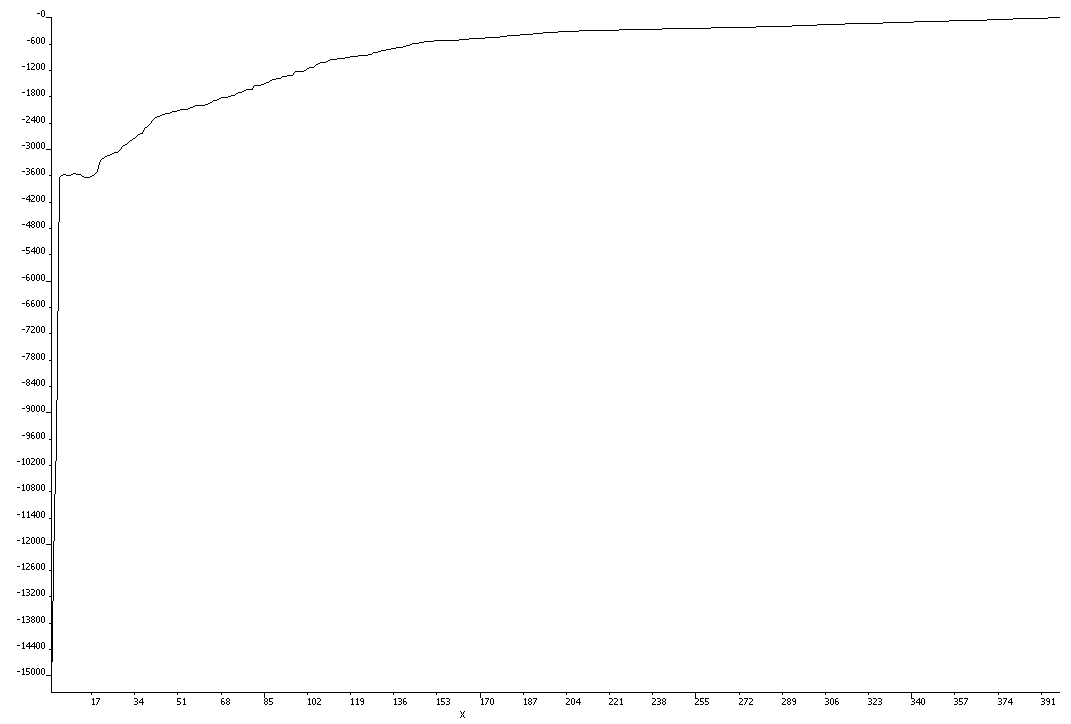
\includegraphics[width=1.0\textwidth]{tgres.png}}
\caption{$\Delta h_n$ per number of topics $n$ when running Topic Grouper on the synthetic data set as described above (Generated with class \texttt{OptimizedTGTester}.)}
\label{impresult}
\end{figure}

\begin{figure}
\center{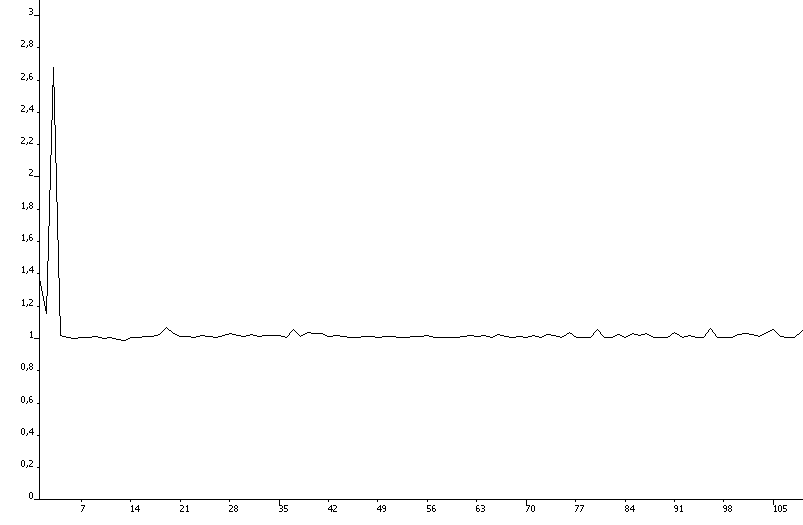
\includegraphics[width=1.0\textwidth]{tgres2.png}}
\caption{$\Delta h_{n-1} / \Delta h_{n}$ per number of topics $n$ when running Topic Grouper on the synthetic data set as described above (Generated with class \texttt{OptimizedTGTester2}.)}
\label{impresult2}
\end{figure}

The first four lines of Figure \ref{tgresult} show the top ten words as computed for each topic via Topic Grouper at $n = 4$. In this case, the words per topic are sorted by the frequency in the document collection (as shown in parentheses). All words were assigned correctly. Although not shown, this also holds for most lower ranked words. Errors occur at lower frequencies usually because those frequencies are not significant anymore (i.e., they do not correspond to their true generative probabilities due to the small size of the data set).

The last line of Figure \ref{tgresult} shows the counts $f(t_i)$ for each of the computed topics $t_1,\ldots,t_4$. The frequencies closely match the ratio of the prior $\alpha = (5, 0.5, 0.5, 0.5)^\top$ used at the generation of data set. In other words: Topic Grouper could be applied as preprocessing procedure for LDA in order to find reasonable hyperparameters for $n$ and $\alpha$.

Note that we have tried many other variations when parametrizing the generation of the synthetic data set including other document sizes (that also vary across documents), larger document collections, more topics, other $\alpha$-priors an so on. The results reported above are representative in a sense that all data set variations led to similar results and conclusions.

\begin{figure}
{\tiny
\begin{verbatim}
[61 (2471), 30 (2421), 39 (2399), 98 (2396), 58 (2317), 18 (2303), 60 (2294), 46 (2285), 33 (2285), 27 (2282) ...
[172 (281), 148 (277), 116 (270), 184 (270), 158 (257), 193 (253), 176 (252), 111 (251), 144 (246), 119 (243) ...
[317 (301), 368 (291), 379 (290), 364 (280), 315 (277), 324 (267), 319 (262), 307 (261), 304 (254), 343 (247) ...
[219 (267), 262 (250), 212 (250), 283 (249), 208 (248), 200 (247), 273 (243), 235 (241), 214 (236), 269 (236),...
Topic frequencies: [138856 14460 13236 13448 ]\end{verbatim}}
\caption{Result of running Topic Grouper on the synthetic data set as described above (Generated with class \texttt{OptimizedTGTester}.)}
\label{tgresult}
\end{figure}

\subsubsection{Data Set with Topical Homonyms}

\subsection{Perplexity Analysis}

We apply \textit{perplexity} as discussed in \cite{Blei:2003:LDA:944919.944937} to a test collection $D_{test}$, which is defined as:

\[ perplexity(D_{test}) := \exp (- \sum_{d \in D_{test}} \log p(d) / \sum_{d \in D_{test}} |d| )\]

Using topic modeling the document probability $p(d)$ under a (trained) topic model should be determined as follows:

\[p(d) = (|d|! / \prod_{w \in V, f_d(w) > 0} f_d(w)!) \cdot \prod_{w \in V, f_d(w) > 0} p(w|d),\] 
\[p(w|d) = (\sum_{t \in T} p(w|t) \cdot p(t|d))^{f_d(w)}.\]

The expression $|d|! / \prod_{w \in V, f_d(w) > 0} f_d(w)!$ accounts for the underlying bag of words model for documents (where word order is ignored).
Not that the size of a test document $|d| = \sum_{w \in V} f_d(w)$ is measured only with words from training vocabulary $V$.

Regarding Topic Grouper, the probability $p(w|d)$ can be estimated as follows on the basis of a partitioning $T(n)$ and the maximum likelihood estimations for $p(t|d)$ and $p(w|t)$ from equation \ref{sn}:

\[ p(w|d) \approx (f(w) / f(t(w)) \cdot f_d(t(w)) / |d|)^{f_d(w)}.\]

Note that $f_d$ and $|d|$ refer to $D_{test}$ whereas $t(w)$, $f(w)$, $f(t)$ and $V$ belong to the model (i.e., the partitioning $T(n)$ of $V$ into topics) and the training collection $D$ respectively.  Also note that the sum over all topics ${t \in T}$ from above has only one non-zero addend because $p(w|t) = 0$ if $w \notin t$.

The estimation has to extreme cases: If $|T(n)| = 1$, then $p(w|d) \approx (f(w) / \sum_{w \in V} f(w))^{f_d(w)}$ -- this is the unigram model. If $|T(n)| = |V|$, then  $p(w|d) \approx (f_d(w) / |d|)^{f_d(w)}$, which means word probabilities are estimated directly via the test document (and nothing is learned from the training data).

Unfortunately, computing $p(w|d)$ on the basis of an LDA-model is not as straight-forward because $p(t|d)$ from above expression is unknown for test documents $d$.
Theoretical solutions to this issue are discussed in \cite{Wallach:2009:EMT:1553374.1553515}.
We tried Mallet's\footnote{See \href{http://mallet.cs.umass.edu}{http://mallet.cs.umass.edu}.} implementation of the "Left-to-Right" algorithm from \cite{wallach08} in order to compute $\log p(d)$ directly for given a LDA-model and a test document $d$. For reference, we call this approach "LDA-P-Method 1". Unfortunately the implementation seems to be flawed and returned errors during computation.
Apart from this problem, we believe that the approach is generally questionable, since it actually defers a training task (requiring considerable statistical inference efforts) to the evaluation phase.

Another alternative discussed in a forum entry\footnote{See \href{http://stats.stackexchange.com/questions/18167/how-to-calculate-perplexity-of-a-holdout-with-latent-dirichlet-allocation}{{http://stats.stackexchange.com/questions/18167/how-to-calculate-perplexity-of-a-holdout-with-latent-dirichlet-allocation}}.} is to hold out a percentage of words from each training document and then to compute $p(d)$ on the held out words (by considering the set of held out words from each training document as a test document). Consequently, each training document is reduced by the corresponding set of held out words. $p(t|d)$ is then obviously known from the LDA model, since $d$ (or at least parts of it) were used during training. The author of the entry argues that the approach is suboptimal and biased because it does not work with "proper" test documents. For reference we call this approach "\textbf{LDA-P-Method 2}".

We suggest a third alternative which is to estimate $p(t|d)$ on the basis of all distributions available as part of the generated LDA-model itself, namely
$p(w|t)$ and $p(t)$:
\[ p(t|d) \approx 1 / |d| \cdot \sum_{w \in V} f_d(w) \cdot p(t|w)\]
\[ p(t|w) = p(w|t) \cdot p(t) / p(w), p(w) \approx f(w) / \sum_{w \in V} f(w)\]
So $p(t|d)$ is averaged across the words in $d$ and "degree to which $t$ belongs to each $w$".
We think this is "fair game" because it makes best use of the model and also, there is no need to create questionable holdout documents as discussed in the forum entry. For reference we call this approach "\textbf{LDA-P-Method 3}".

Figure \ref{perplexity1} depicts a perplexity graph for Topic Grouper regarding the data set from Section \ref{twcdataeval} and a randomized holdout set for test with 10\% of the size of the entire data set (so only 90\% used for training). The X axis represents the number of topics.
The perplexity at $n = 4$ is about $13.998$.

\begin{figure}
\center{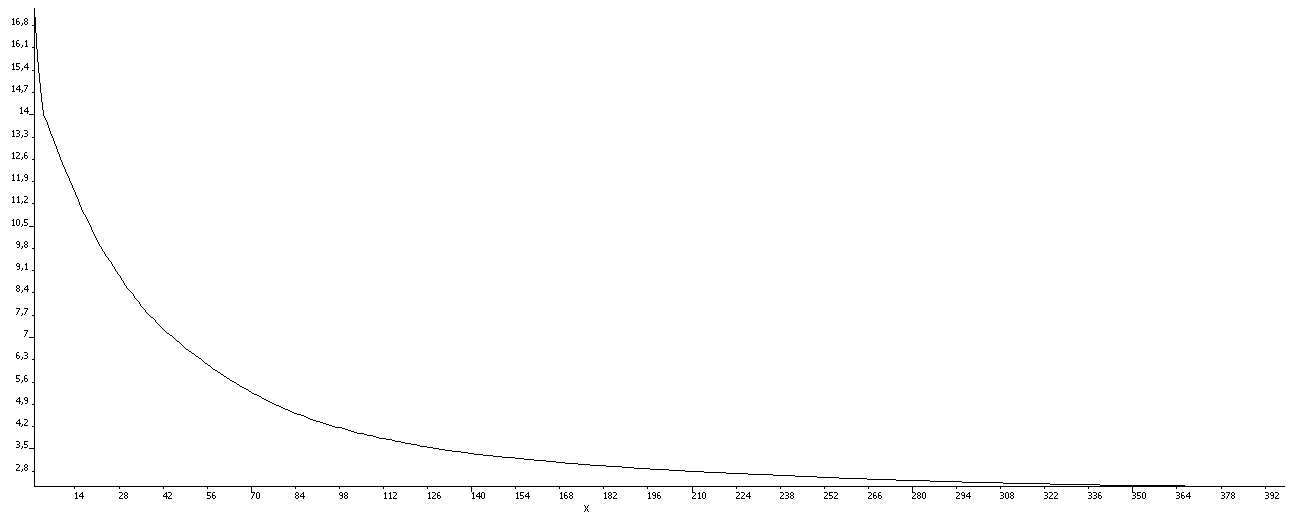
\includegraphics[width=1.0\textwidth]{perplexity1.png}}
\caption{Perplexity as a result of Topic Grouper on the data set from Section \ref{twcdataeval} but with a 10\% holdout for test (Generated with class \texttt{OptimizedTGTesterPM3}.)}
\label{perplexity1}
\end{figure}

Figure \ref{perplexity2} depicts a perplexity graph for LDA using LDA-P-Method 3 regarding the same data set as in Figure \ref{perplexity1}. LDA hyperparameters are set (in favour of LDA) to the best matching values, which are $n = 4$, $\alpha = (5, 0.5, 0.5, 0.5)^\top$ and $\beta=0.5$. The X axis represents number of iterations. The perplexity is about $15.944$ after 400 iterations .

\begin{figure}
\center{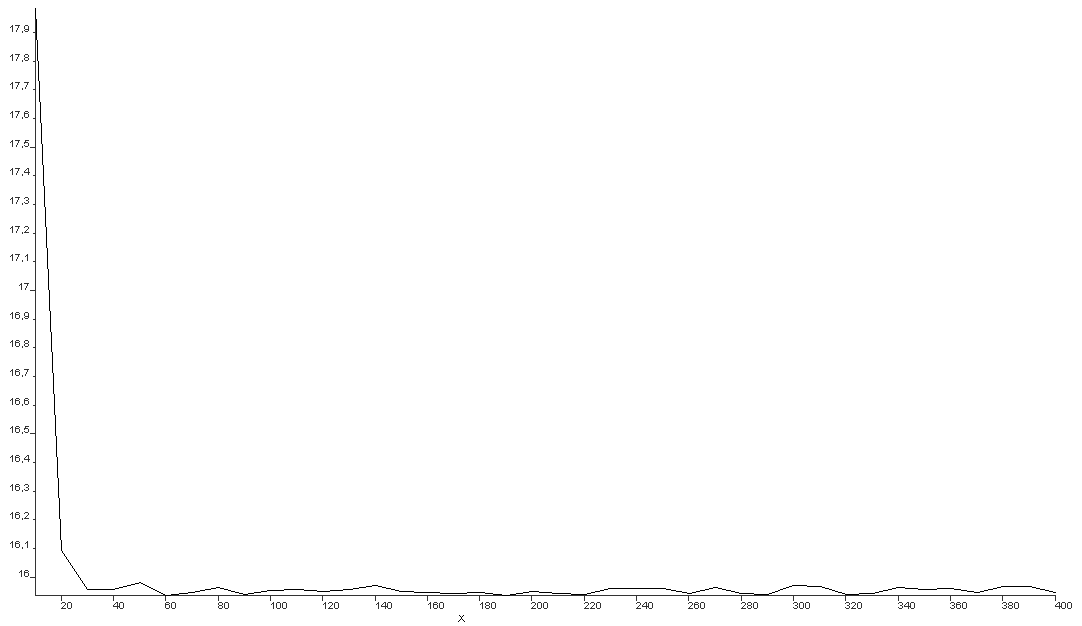
\includegraphics[width=1.0\textwidth]{perplexity2.png}}
\caption{Perplexity as a result of LDA on the data set from Section \ref{twcdataeval} but with a 10\% holdout for test (using LDA-P-Method 3) (Generated with class \texttt{AsymmetricLDAGibbsTesterPM3}.)}
\label{perplexity2}
\end{figure}

We also tested LDA-P-Method 2 and constructed the holdout set and training set accordingly. Figures \ref{perplexity3} and \ref{perplexity4} show the corresponding results on the data set from Section \ref{twcdataeval} but with 300 instead of 30 words per documents instead. (We had to increase the document size so that the holdout documents end up to have a reasonable size of about 30 words.) The perplexity for Topic Grouper is about 13.589 at $n = 4$ and about $15.417$ for LDA after 400 iterations.

\begin{figure}
\center{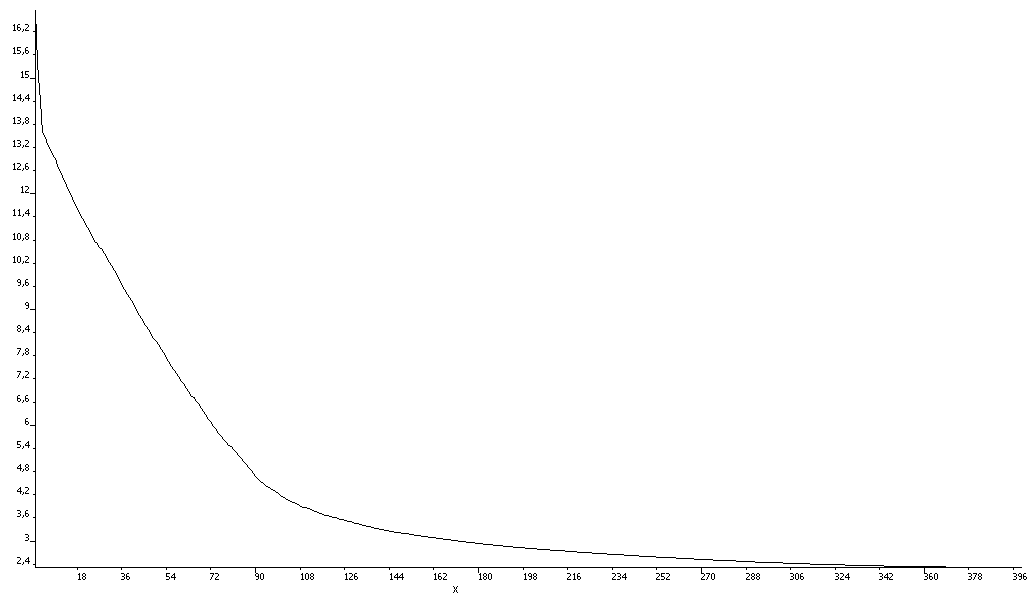
\includegraphics[width=1.0\textwidth]{perplexity3.png}}
\caption{Perplexity as a result of Topic Grouper on the data set from Section \ref{twcdataeval} but with a 10\% holdout for test. The holdout is constructed according to LDA-P-Method 2 (Generated with class \texttt{OptimizedTGTesterPM2}.)}
\label{perplexity3}
\end{figure}

\begin{figure}
\center{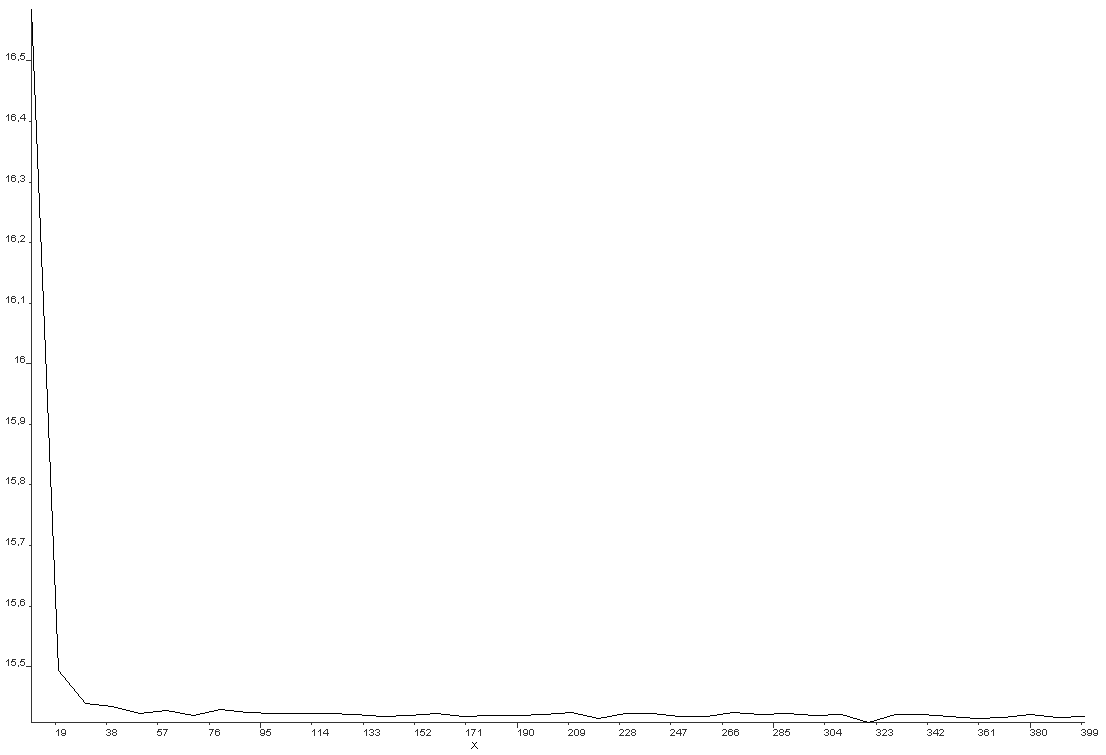
\includegraphics[width=1.0\textwidth]{perplexity4.png}}
\caption{Perplexity as a result of LDA on the data set from Section \ref{twcdataeval} but with a 10\% holdout for test (using LDA-P-Method 2). The holdout is constructed according to LDA-P-Method 2 (Generated with class \texttt{AsymmetricLDAGibbsTesterPM2}.)}
\label{perplexity4}
\end{figure}


\subsection{Result Visualization and Inspection}

Since Topic Grouper is essentially an agglomerative clustering approach, all respective visualization techniques become available.
E.g., Figure \ref{dendrogram} shows a corresponding dendrogram for the data set from Section \ref{twcdataeval}, but with only 40 instead of 400 words (just to simplify the diagram).
 
\begin{figure}
\center{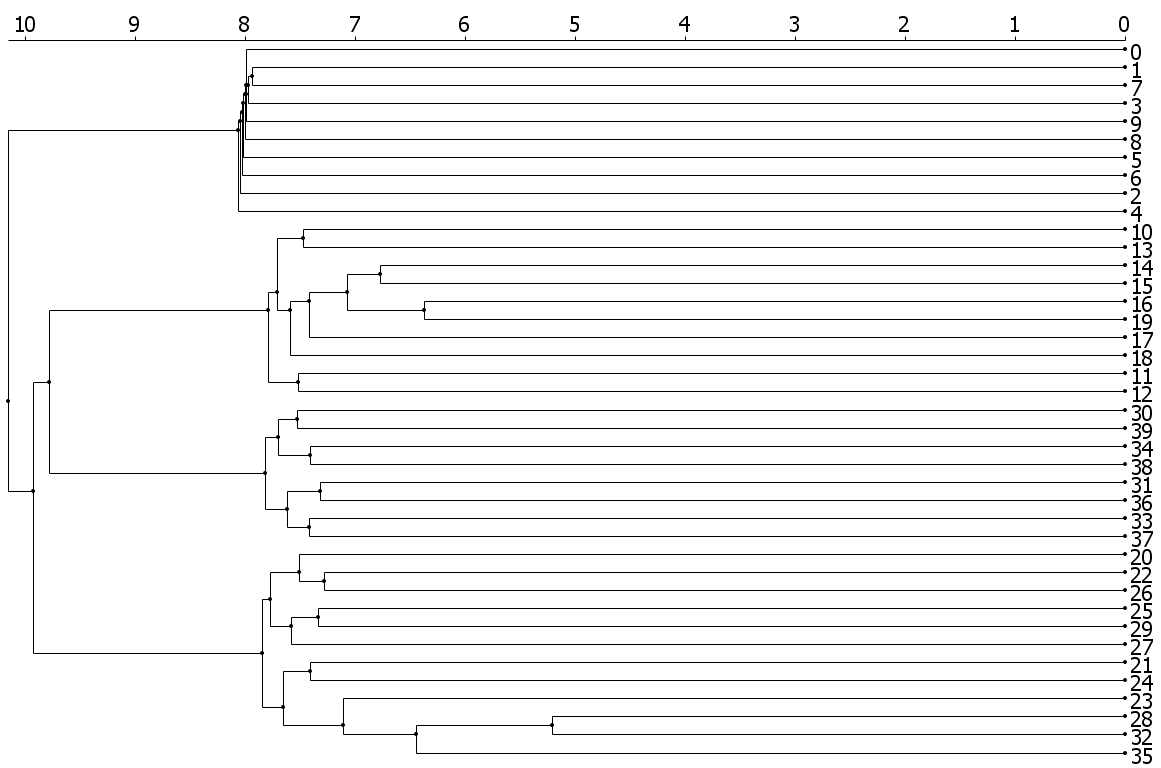
\includegraphics[width=1.0\textwidth]{dendrogram.png}}
\caption{Dendrogram as a result of Topic Grouper on a synthetic data set according to Section \ref{twcdataeval} but with only 40 words; the X axis  depicts the values of $\log - \Delta h_{n}$ (Generated with class \texttt{DendroGramDemo}.)}
\label{dendrogram}
\end{figure}

As opposed to LDA, Topic Grouper returns a hierarchical topic model by design.
This quality can be used to do interactive "drill downs" from larger to smaller topics assuming that larger topics form some kind semantic abstraction of contained smaller topic and also, contained topics are specializations of containing topics. To get an idea of the meaning of a topic, every topic can be represented by its top-most frequent words on every containment level.
Analyzing results this way may give users additional insight into the nature of a document collection's inherent topics.

We created corresponding mind map diagrams by exporting computation results of Topic Grouper to the mind map tool FreeMind
\footnote{See \href{http://freemind.sourceforge.net}{http://freemind.sourceforge.net}.}. (To do so, we simply generated appropriate XML files, which are FreeMind's standard file format.) More frequent word sets are shaded in blue (because they tend to be less relevant, e.g. when thinking of stop words), whereas less frequent word are shaded in red. Moreover, tree nodes are marked with a yellow flag if 
$\Delta h_{n-1} / \Delta h_{n}$ exceeded an adjustable threshhold (in this case set to 1.2) (see also Figure \ref{impresult2} for reference).
The yellow flags indicate joins that lead to "unusually high cost", which is a hint that two related topics have distinct semantics.

Note that corresponding topics may occur further up or deeper down in the mind map. This makes the visualization technique rather independent of a specific fixed number topics $n$ to be considered at a time (as is custom with LDA). The appeal to the user is rather: "Look where the yellow flags are and see if you can make sense of the topics described via the words at the corresponding nodes."

Figure \ref{mindmap1} presents a corresponding mind map in analogy to Figure \ref{dendrogram}.
\begin{figure}
\center{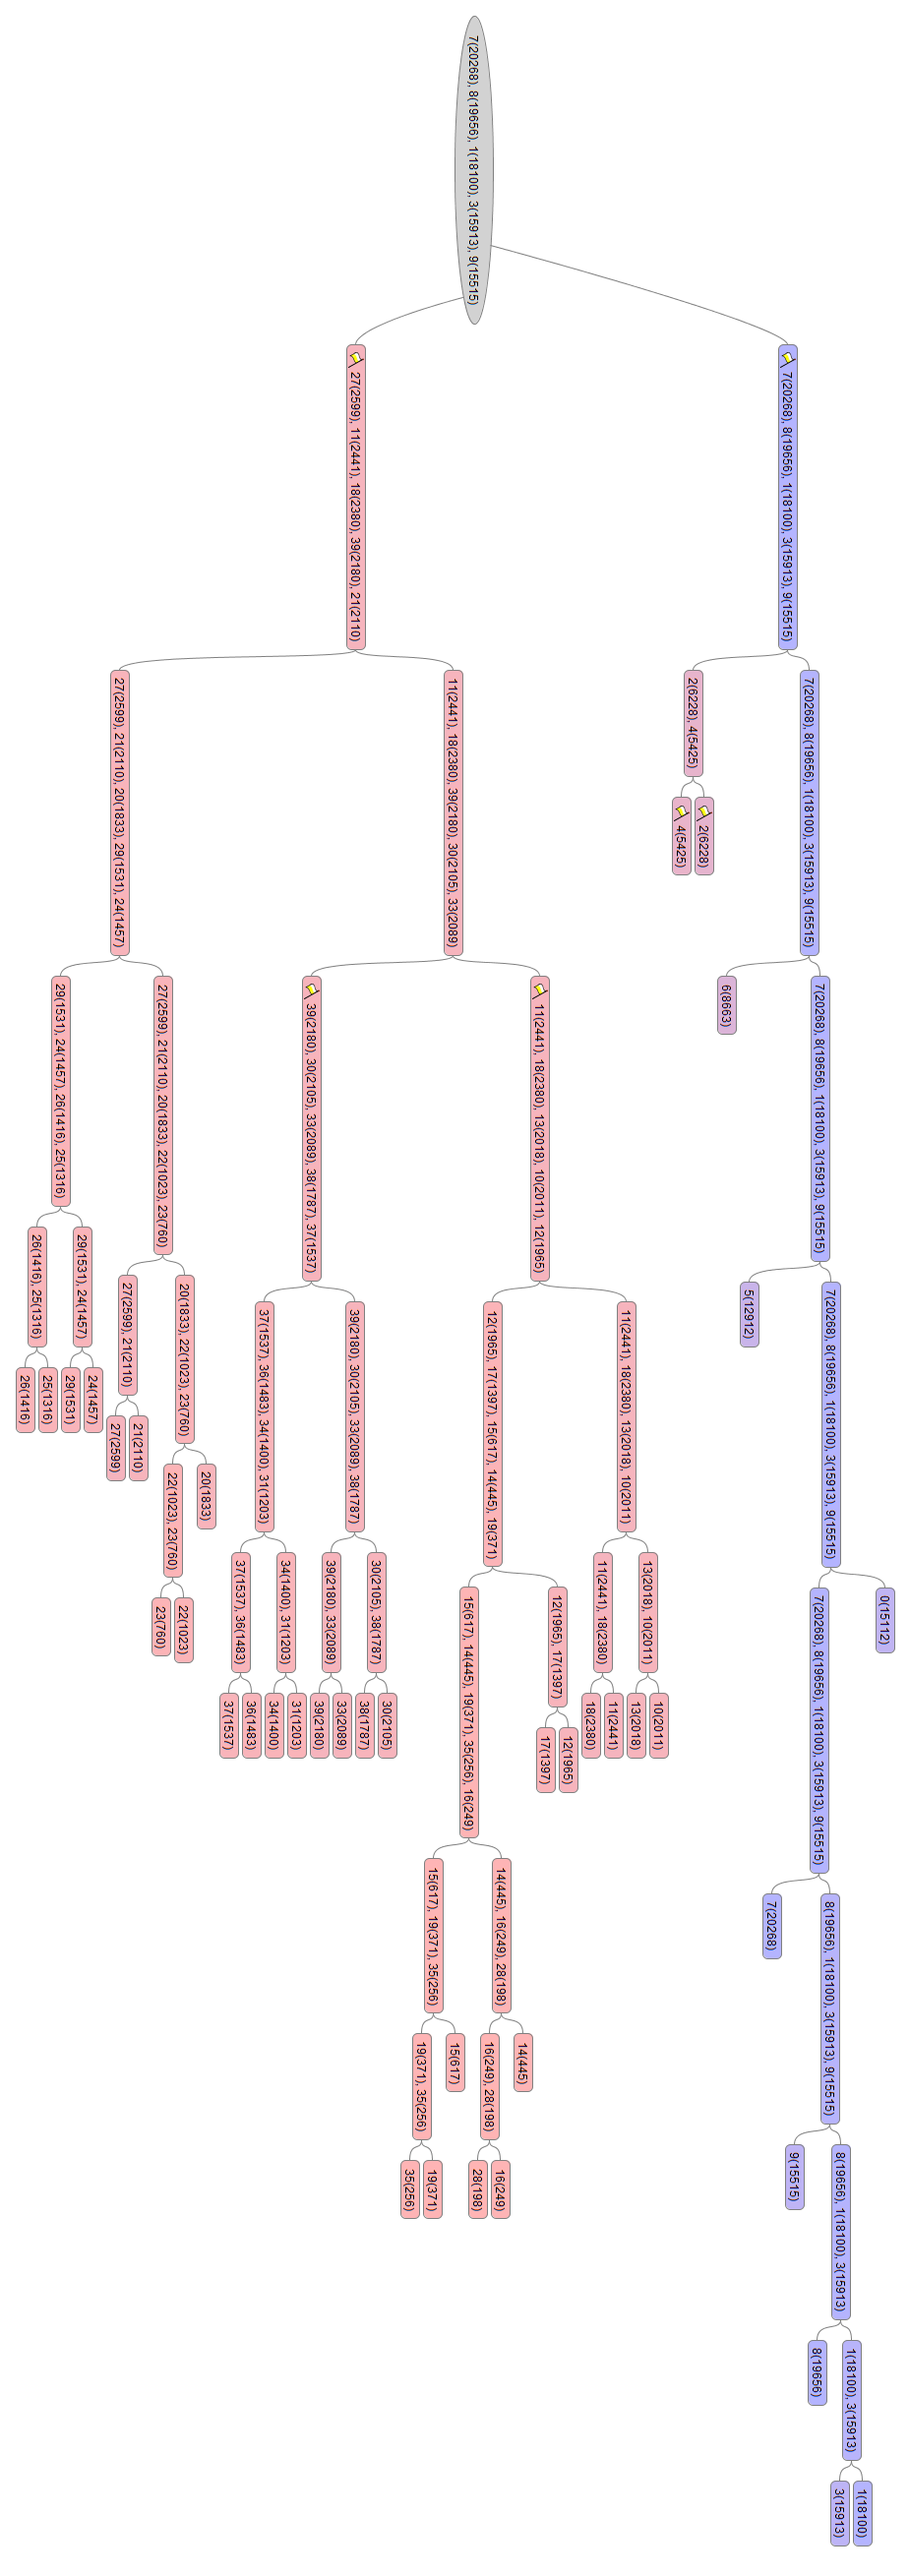
\includegraphics[height=1.0\textheight]{mindmap1.png}}
\caption{Mind map as a result of Topic Grouper on a synthetic data set according to Section \ref{twcdataeval} but with only 40 words (Generated with class \texttt{MindMapDemo}.)}
\label{mindmap1}
\end{figure}

For a more realistic mind map, we ran Topic Grouper on a subset of the (supposedly well known) Reuters 21578 data set\footnote{See
\href{http://www.daviddlewis.com/resources/testcollections/reuters21578/}{http://www.daviddlewis.com/resources/testcollections/reuters21578/}.}.
We used a subset of 13476 documents, performed stemming (using a Porter stemmer), kept stop words and removed all terms with a frequency less than 50, which resulted in $|V| = 2343$. Figure \ref{mindmap2} shows an extract of the resulting mind map. Many more detailed nodes have been collapsed after inspection to get a reasonably sized image.

\begin{figure}
\center{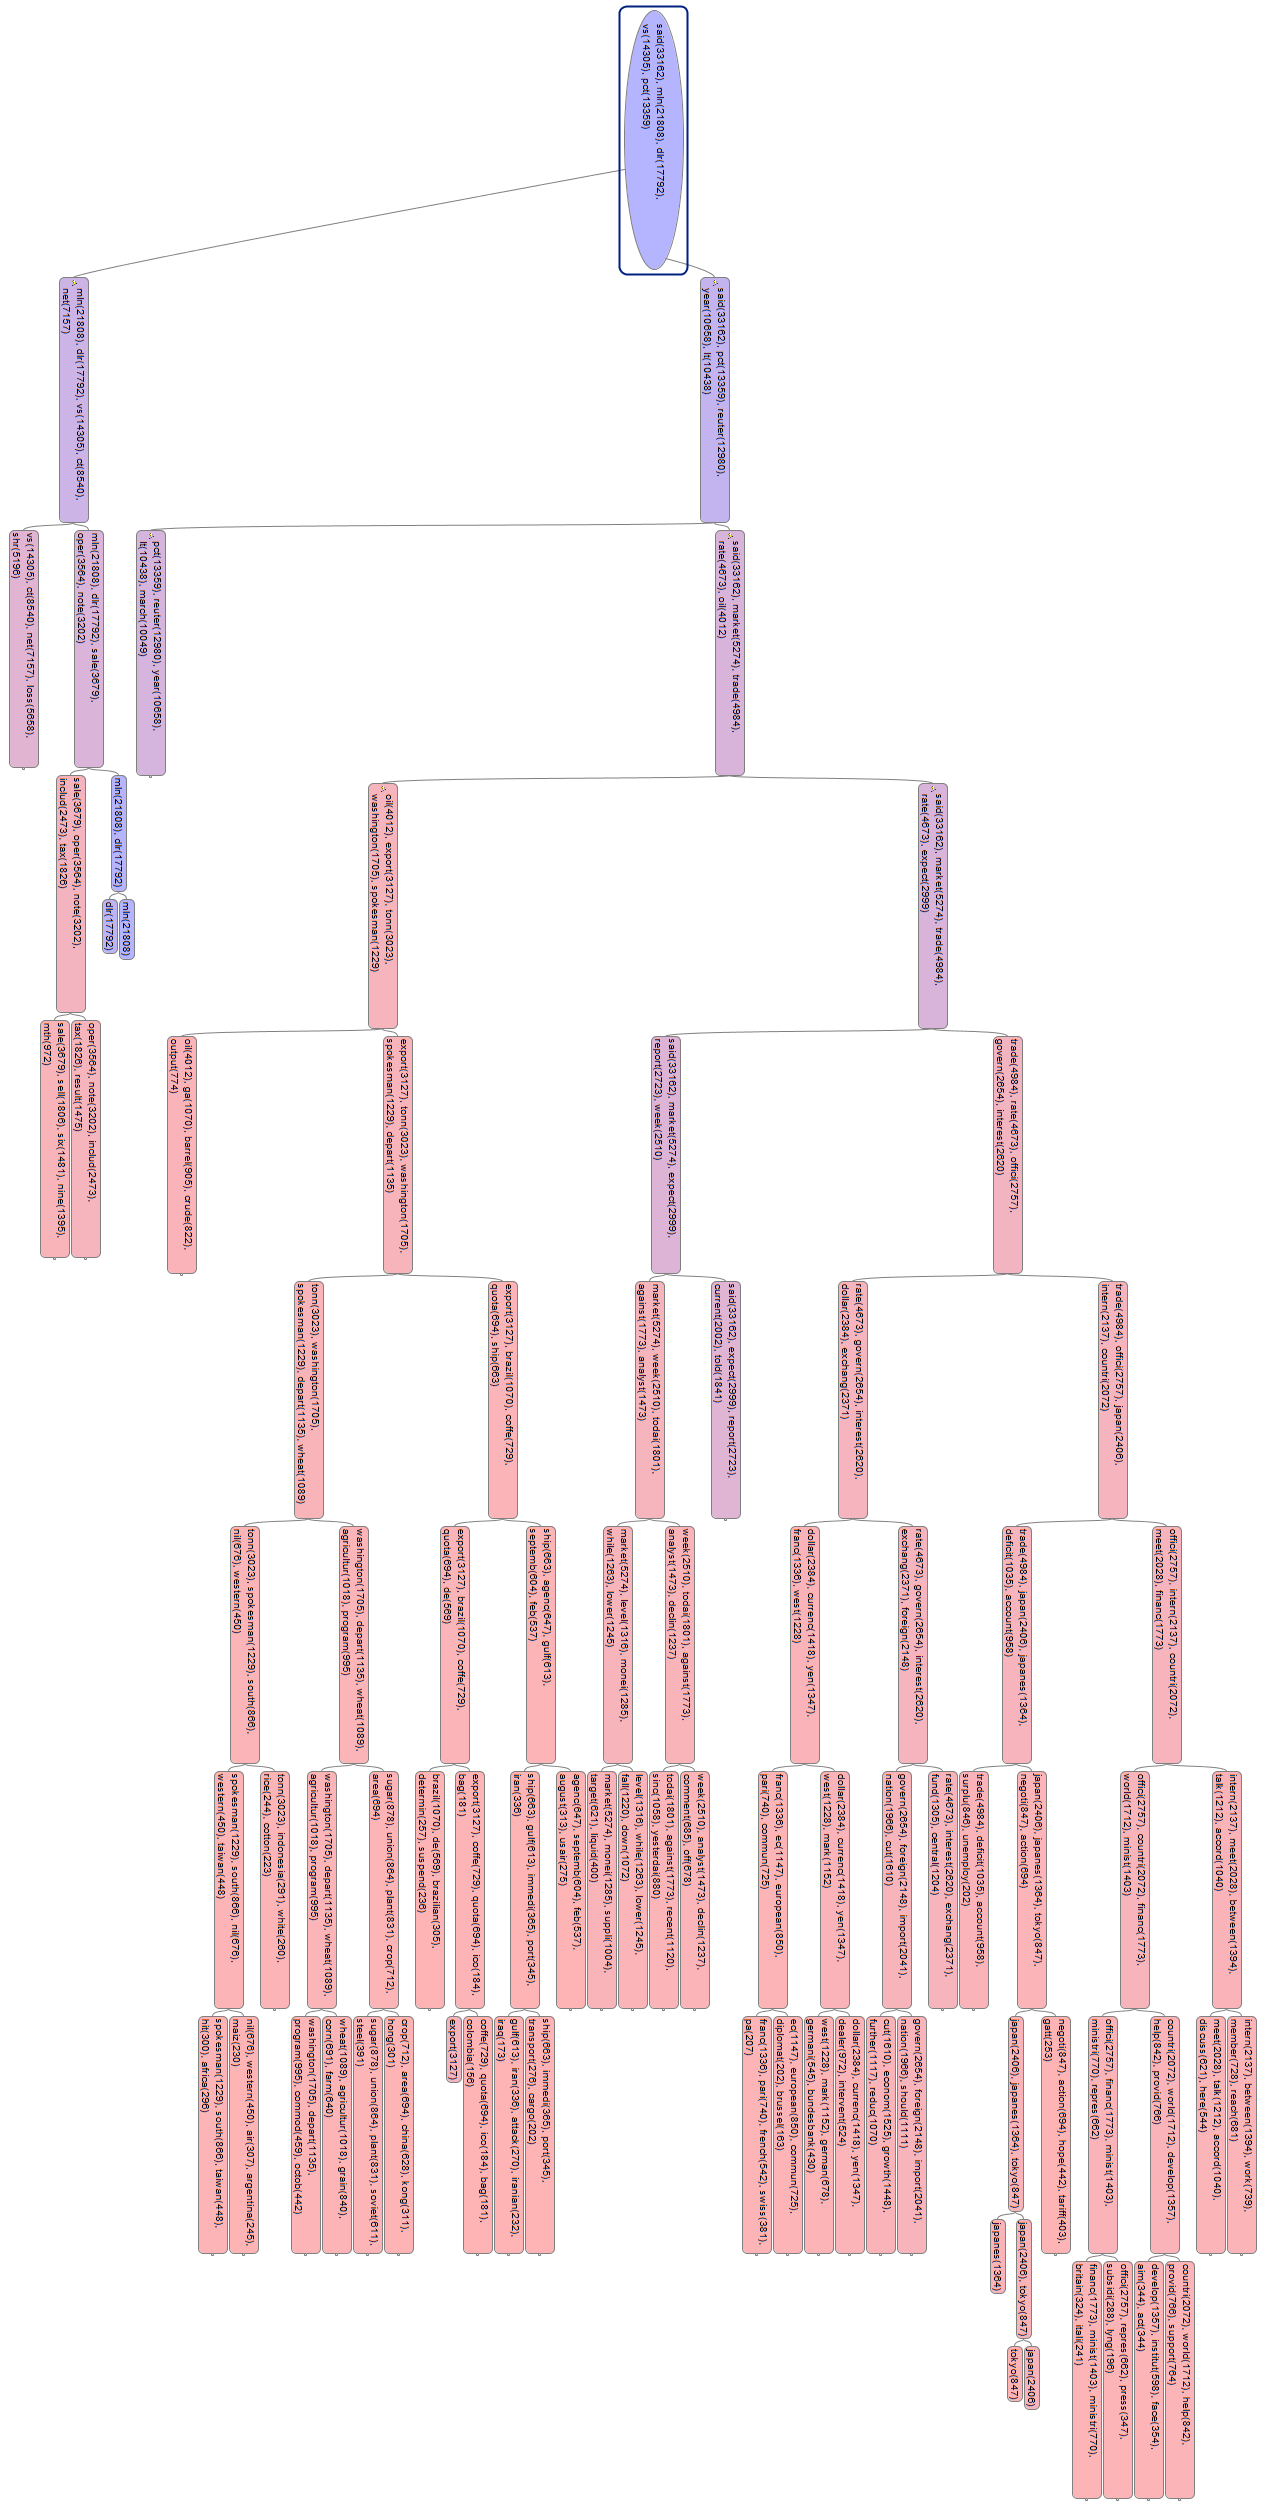
\includegraphics[height=1.0\textheight]{mindmap4.png}}
\caption{Mind map as a result of Topic Grouper on a subset of the Reuters 21578 data set. (Generated with class \texttt{MindMapDemoReuters}.)}
\label{mindmap1}
\end{figure}

\section{Implementation}

A basic Java implementation of Topic Grouper is available under\\
\href{https://github.com/pfeiferd/TopicGrouperJ}{https://github.com/pfeiferd/TopicGrouperJ}.
Required libraries first must be included by running Maven\footnote{See \href{https://maven.apache.org/}{https://maven.apache.org/}.} on \texttt{./pom.xml}.

The main methods of classes in the package \texttt{org.hhn.topicgrouper.figures} can be used to generate \emph{all} the figures of this document.
(The unqualified Java name of a corresponding class is mentioned in each figure's caption.)
All output files can be found in the folder \texttt{./target} (if not present, it must be created first).
LDA outputs its topics in files like \texttt{./target/*.topWords}.
The mind maps are generated as XML files like \texttt{./target/*.mm} and can be opened with the open source tool FreeMind for display.
Other graphs and charts appear in a window while running Topic Grouper (or LDA) and are updated during the run.
Textual outputs of Topic Grouper appear on the command line or in a files like \texttt{./target/*.txt}.

To run programs related to the Reuters 21578 data set, the corresponding data set files must first be downloaded and placed in the folder
\texttt{./src/main/resources/reuters21578}. There is a read-me file in that folder, that explains the details.
Note that the library \texttt{./lib/lingpipe-3.9.3.jar} is required on your class path in order to read an tokenize the Reuters documents. (Unfortunately, the library cannot be downloaded from the Internet via Maven.)


\nocite{*} %Auch nicht-zitierte BibTeX-Einträge werden angezeigt.
\bibliographystyle{apalike} %Art der Ausgabe: plain / apalike / amsalpha / ...
\bibliography{literature} %Eine Datei 'literatur.bib' wird hierfür benötigt.


\end{document}